\section{A Potential Spectral Path Towards the Riemann Hypothesis}
\vspace{10pt}

The framework presented suggests a potential path towards a spectral proof of the Riemann Hypothesis. If the constructed operator \( \hat{H}_\infty \) (the hypothesized infinite-dimensional limit) possesses certain ideal properties, it could lead to the RH. Specifically, the following conditions would need to be rigorously proven:
\begin{enumerate}
    \item \textbf{Exact Spectral Alignment:} The eigenvalues \( \lambda_n \) of the rigorously defined, self-adjoint operator \( \hat{H}_\infty \) must coincide exactly with the imaginary parts \( \gamma_n \) of the non-trivial Riemann zeros:
    \[
    \text{Spectrum}(\hat{H}_\infty) = \{ \gamma_n \mid \zeta(1/2 + i \gamma_n) = 0 \}.
    \]
    \item \textbf{Operator Zeta Function Properties:} The associated operator zeta function \( \zeta_{\hat{H}}(s) = \operatorname{Tr}(\hat{H}_\infty^{-s}) \) must be shown to admit meromorphic continuation to the entire complex plane.
    \item \textbf{Functional Equation and Equivalence:} It would need to be proven that the completed operator zeta function \( \xi_{\hat{H}}(s) \) satisfies the same functional equation as the Riemann xi-function, \( \xi_{\hat{H}}(s) = \xi_{\hat{H}}(1 - s) \), and ultimately that \( \zeta_{\hat{H}}(s) \equiv \zeta(s) \).
\end{enumerate}
Establishing these points through rigorous mathematical proof would validate this spectral approach and consequently affirm the Riemann Hypothesis. However, achieving these proofs remains a significant open challenge.

\subsection*{Next Steps}
\begin{itemize}
  \item Prove convergence and analytic continuation of \( \zeta_{\hat{H}}(s) \),
  \item Rigorously derive spectral alignment \( \lambda_n = \gamma_n \),
  \item Demonstrate uniqueness of \( \hat{H}_\infty \) as a spectral generator of \( \zeta(s) \).
\end{itemize}

\begin{figure}[h]
\centering
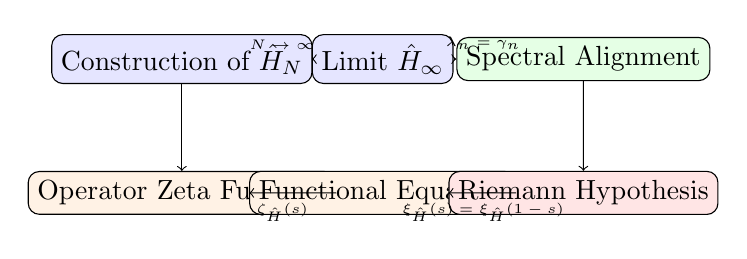
\begin{tikzpicture}[scale=0.85]
    % Draw a roadmap of the proof strategy
    % Draw stages as nodes
    \node[draw, rounded corners, fill=blue!10] (construction) at (0,0) {Construction of $\hat{H}_N$};
    \node[draw, rounded corners, fill=blue!10] (limit) at (3,0) {Limit $\hat{H}_\infty$};
    \node[draw, rounded corners, fill=green!10] (spectral) at (6,0) {Spectral Alignment};
    
    \node[draw, rounded corners, fill=orange!10] (zeta) at (0,-2) {Operator Zeta Function};
    \node[draw, rounded corners, fill=orange!10] (functional) at (3,-2) {Functional Equation};
    \node[draw, rounded corners, fill=red!10] (rh) at (6,-2) {Riemann Hypothesis};
    
    % Draw arrows connecting nodes
    \draw[->] (construction) -- (limit);
    \draw[->] (limit) -- (spectral);
    \draw[->] (construction) -- (zeta);
    \draw[->] (zeta) -- (functional);
    \draw[->] (spectral) -- (rh);
    \draw[->] (functional) -- (rh);
    
    % Add descriptive text
    \node[above] at (1.5,0) {\tiny $N \to \infty$};
    \node[above] at (4.5,0) {\tiny $\lambda_n = \gamma_n$};
    \node[below] at (1.5,-2) {\tiny $\zeta_{\hat{H}}(s)$};
    \node[below] at (4.5,-2) {\tiny $\xi_{\hat{H}}(s) = \xi_{\hat{H}}(1-s)$};
\end{tikzpicture}
\caption{A roadmap showing the logical flow from operator construction to a potential proof of the Riemann Hypothesis.}
\label{fig:roadmap}
\end{figure}